\subsubsection{PCM}
$PCM$ is a cluster of shared memory machines, thus all considerations regarding mapping of processes to cores made in~\ref{fram-intr} become matter of study. Even the official guide of \textit{mvapich2}, the version of MPI that we have used to exploit Infiniband, emphasizes the importance of process-to-core mapping: as shown in~\cite{MVAPICH2-MAPPING}, different allocations of processes to cores can have a significant impact on the cost of communications. In principle, an entire study could be dedicated to this topic, leading to a lot of possible mappings, each one based on its reasonable heuristic. Obviously, we had to limit our analysis to a subset of the most simple mappings. In particular, we have studied the following configurations:   
\begin{itemize}
\item \textbf{Sequential mapping}. Adjacent ranks mapped on adjacent \textit{cores}. E.g., given two CPUs each one with 4 cores and 8 MPI processes, rank 0 goes on the first core of the \textit{first} CPU, rank 1 goes on the second core of the \textit{first} CPU, ..., rank 5 goes on the first core of the \textit{second} CPU and so on.
\item \textbf{Interleaved mapping}. Adjacent ranks mapped on adjacent \textit{CPUs}. E.g., given two CPUs each one with 4 cores and 8 MPI processes, rank 0 goes on the first core of the \textit{first} CPU, rank 1 goes on the first core of the \textit{second} CPU, rank 2 goes on the second core of the \textit{first} CPU and so on.
\item \textbf{Algorithm-specific mapping}. We have also studied a few mapping based on the nature of a specific Sorting Algorithm, like \textit{Mergesort} and \textit{Quicksort}. For instance, a mapping could be designed to let the most critical part of a stencil to take place in shared memory rather than inter-node.  
\end{itemize}
In the following, we will consider only the \textit{sequential mapping} because we have practically experienced that collective communications (in particular, the \textit{gather}) are \textit{extremely} more cost-effective than for other mappings. For more informations about the results obtained with other mappings the reader could refer to the specific material attached to this report.


\begin{figure}[t]
    \begin{center}
        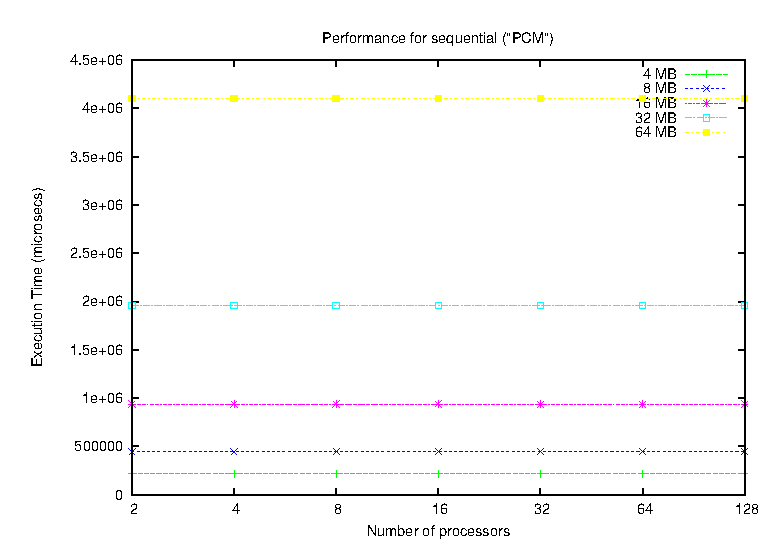
\includegraphics[scale=0.6]{plots/test_01_PCM/NxTxM/sequential_PCM_NxTxM_small}
    \end{center}
    
    \begin{center}
        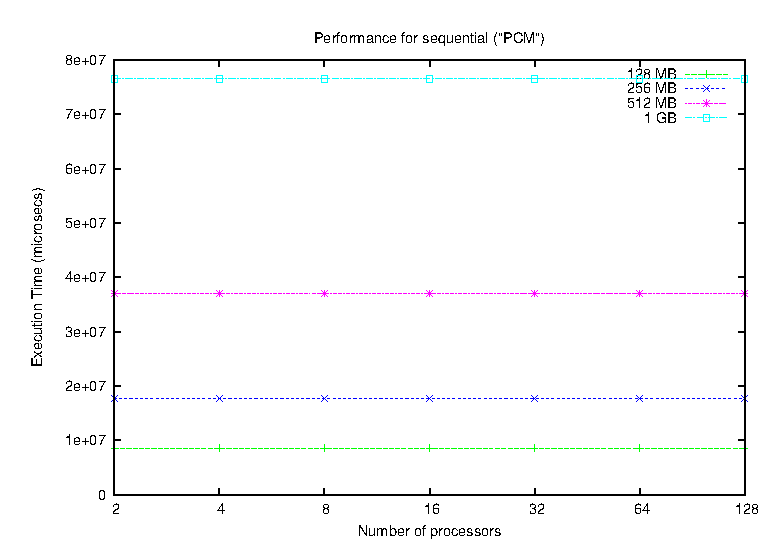
\includegraphics[scale=0.6]{plots/test_01_PCM/NxTxM/sequential_PCM_NxTxM_large}
    \end{center}
    
    \begin{center}
        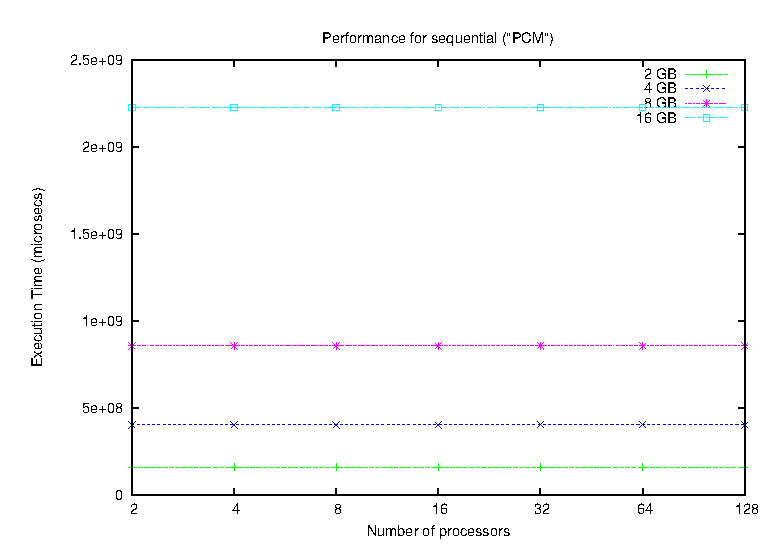
\includegraphics[scale=0.6]{plots/test_01_PCM/NxTxM/sequential_PCM_NxTxM_huge}
    \end{center}
    \caption{\textit{PCM}. Completion Time for the Sequentialsort.}
    \label{sequential-PCM}
\end{figure}

\paragraph{Scalability of Sorting Algorithms}
Unfortunately, we have not been able to run tests for larger data sets due to lack of both time (just testing \textit{Sequentialsort} for a $X$ GBs data set can take either a few minutes or even hours, when $X > 10$) and accessibility to the cluster (we could not keep turned on more than roughly 10 nodes at a time for long, because of the overheating). For instance, if we wanted to test just the data set of 32 GB, we would have to run \textit{every} Sorting Algorithm, for \textit{every} parallelism degree, for some different seeds: this means executing about a hundred of tests, each one taking minutes or maybe hours!  

Figure~\ref{NxTxM} and~\ref{MxTxN} show the time completion of Sorting Algorithms for data sets up to 16 GB. The first interesting result is that all Sorting Algorithms, except \textit{K-Way Mergesort} ($K=4$), reduce the time spent by the \textit{Sequentialsort}. This is true for every data set, even the smallest one; further, the higher is the parallelism degree (in general, at most up to $n=64$) the larger is the gain. Obvioulsy, the larger is the data set, the better is the scalability exhibited by \textit{all} algorithms. Further, notice that while the computational grain increase, the corresponding potential boost of the time spent in communications is kept limited by both the presence of shared memory nodes and the powerful interconnection architecture of $PCM$. One of the several examples that we can do to emphasize this aspect is the following: consider a data set of a certain size, let's say the one of 64M integers (256MB) and focus on a specific Sorting Algorithm, for instance the \textit{Samplesort}. Now, compare Figures~\ref{NxTxA-64M} and~\ref{Pianosa-NxTxA-64M}, where there are shown the time completions for sorting the same data set respectively on $PCM$ and on $Pianosa$: it is clear that, from a \textit{qualitative point of view}, the scalability is greatly more linear on $PCM$ than on $Pianosa$. This is valid also for most of Sorting Algorithms and every data set size. 

Another interesting aspect is the behavior of the algorithms when the parallelism degree $n$ grows from 8 to 16. Some algorithms, like \textit{Samplesort}, \textit{Bucketsort} and \textit{Load-balanced Multi-way Mergesort}, successfully reduce the time completion (but the gain is really far away from the one obtained by passing from $n=4$ to $n=8$); other algorithms either do not improve or even worsen the time completion with respect to parallelism degree 8. In reality, this is not surprising: we recall that a node of $PCM$ is an $IntelXeon\ X5670$, that is a CMP with 12 cores, and we are using the \textit{sequential mapping}; this means that when $n=8$ all communications take place in shared memory, while when $n=16$ they exploit both the shared memory and $Infiniband$. It is true that $Infiniband$ outperforms any other possible interconnection network, but it is also obvious that, in our scenario, it could represent a ''bottleneck'' for those communications on shared memory. 




%%%%%%%%%%%%%%%%%%%%%%%%%%%%%%%%%%%%%%%% Small data set %%%%%%%%%%%%%%%%%%%%%%%%%%%%%%%%%%%%%%%%%%%%%%%%%%%%%%
\begin{figure}[h]
    \centering
    \subfloat[Quicksort.]{\label{NxTxM_small-quicksort}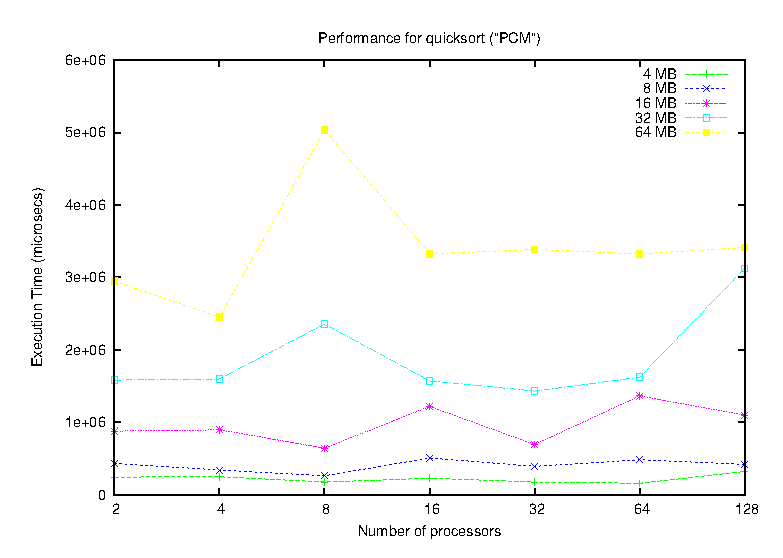
\includegraphics[width=0.4\textwidth]{plots/test_01_PCM/NxTxM/quicksort_PCM_NxTxM_small}} 
    \hspace*{20pt}  
    \subfloat[Bitonicsort.]{\label{NxTxM_small-bitonicsort}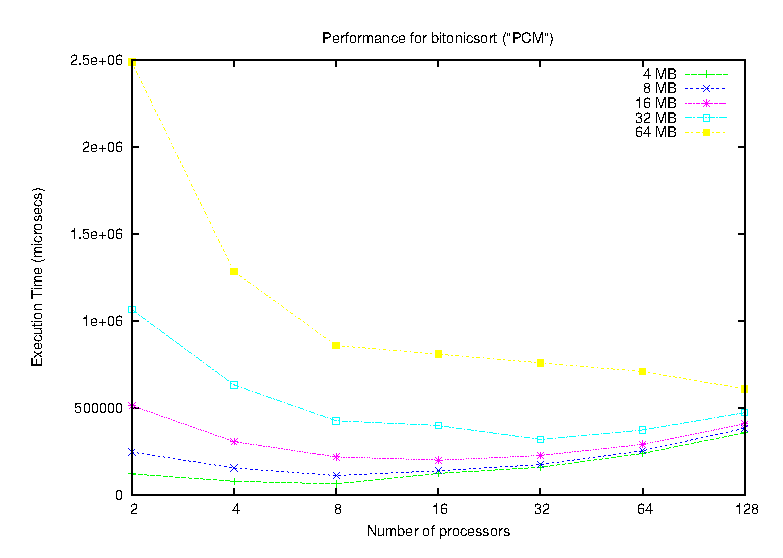
\includegraphics[width=0.4\textwidth]{plots/test_01_PCM/NxTxM/bitonicsort_PCM_NxTxM_small}} 
    
    \centering
    \subfloat[Bucketsort.]{\label{NxTxM_small-bucketsort}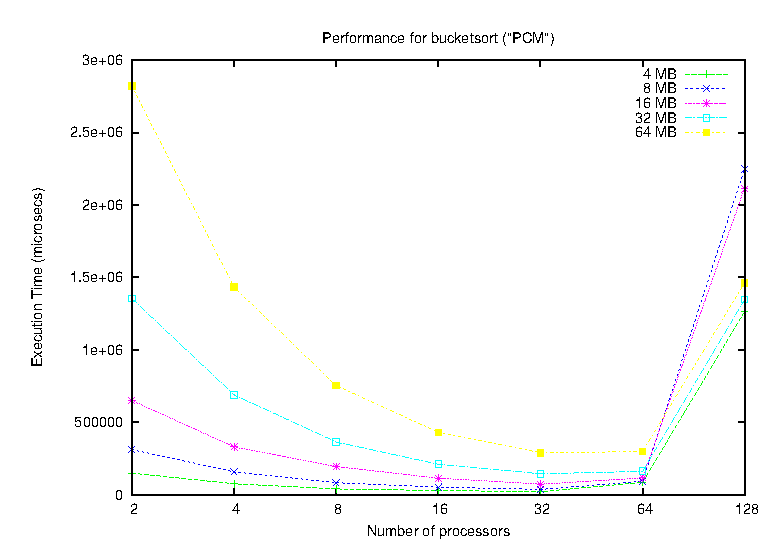
\includegraphics[width=0.4\textwidth]{plots/test_01_PCM/NxTxM/bucketsort_PCM_NxTxM_small}} 
    \hspace*{20pt}
    \subfloat[Samplesort.]{\label{NxTxM_small-samplesort}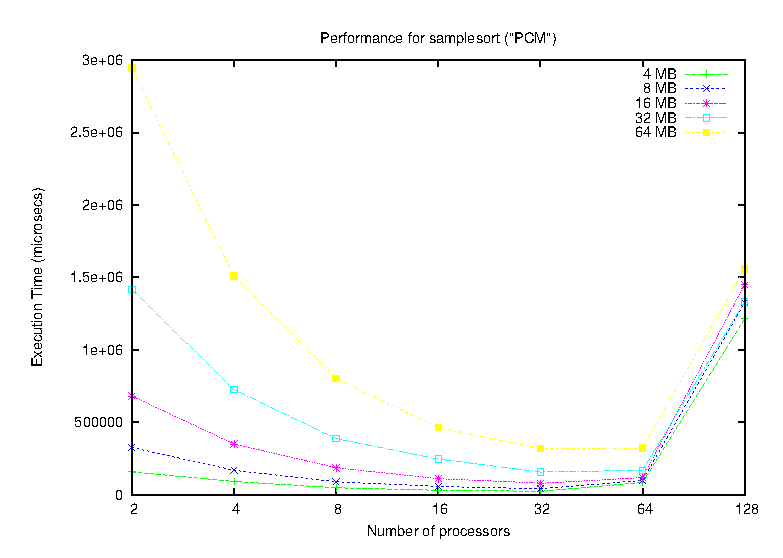
\includegraphics[width=0.4\textwidth]{plots/test_01_PCM/NxTxM/samplesort_PCM_NxTxM_small}} 
    
    \centering
    \subfloat[Mergesort.]{\label{NxTxM_small-mergesort}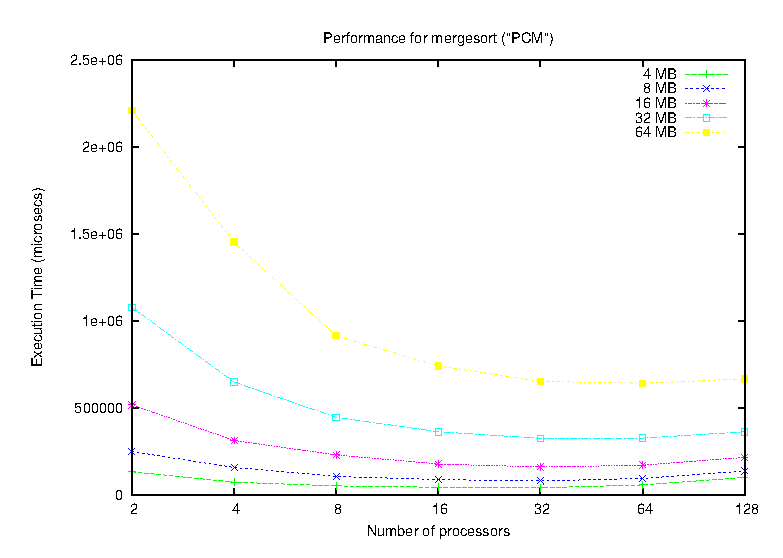
\includegraphics[width=0.4\textwidth]{plots/test_01_PCM/NxTxM/mergesort_PCM_NxTxM_small}}   
    \hspace*{20pt}  
    \subfloat[4-Way Mergesort.]{\label{NxTxM_small-kmerge}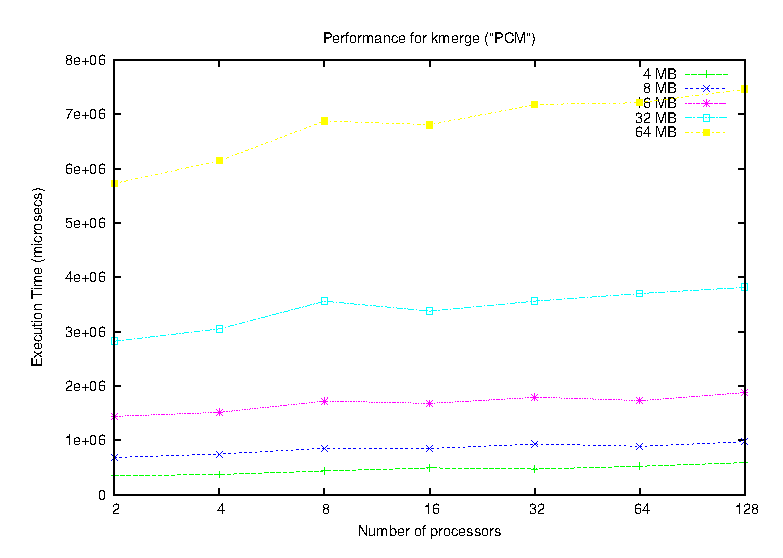
\includegraphics[width=0.4\textwidth]{plots/test_01_PCM/NxTxM/kmerge_PCM_NxTxM_small}} 
    
    \centering
    \subfloat[Load-Balanced Mergesort.]{\label{NxTxM_small-lbmergesort}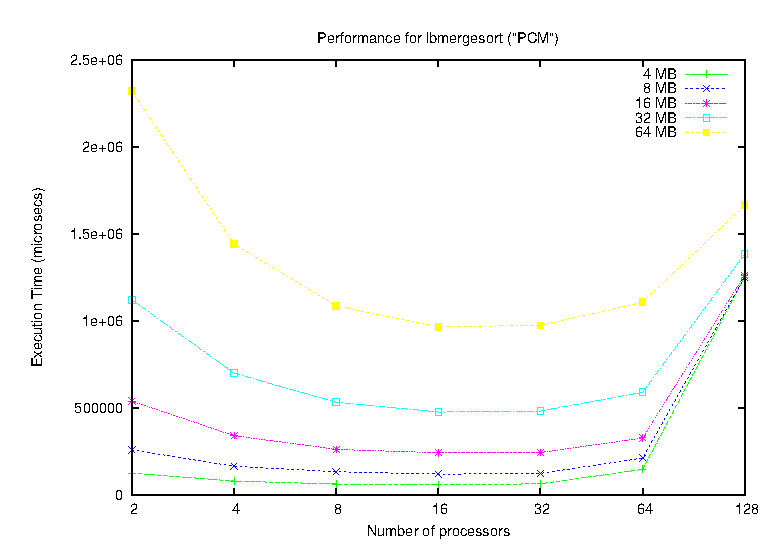
\includegraphics[width=0.4\textwidth]{plots/test_01_PCM/NxTxM/lbmergesort_PCM_NxTxM_small}} 
    \hspace*{20pt}  
    \subfloat[Load-Balanced Multi-Way Mergesort.]{\label{NxTxM_small-lbkmergesort}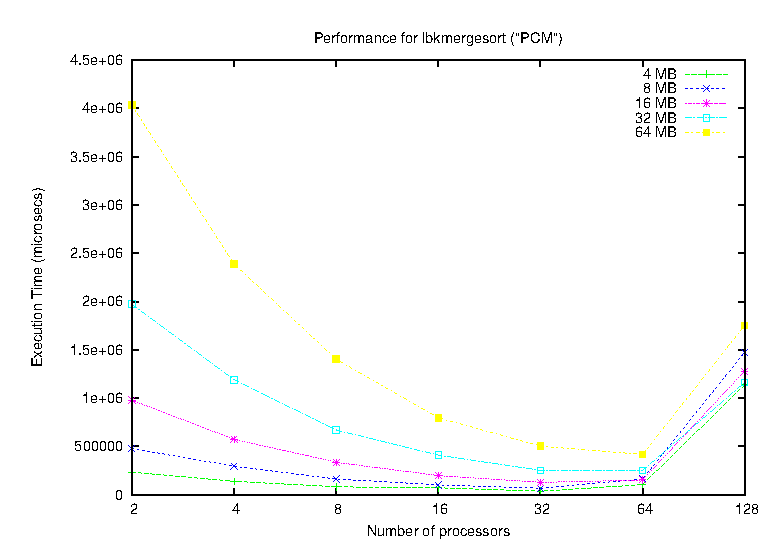
\includegraphics[width=0.4\textwidth]{plots/test_01_PCM/NxTxM/lbkmergesort_PCM_NxTxM_small}}  
    
\end{figure}



  
%%%%%%%%%%%%%%%%%%%%%%%%%%%%%%%%%%%%%%%% Large data set %%%%%%%%%%%%%%%%%%%%%%%%%%%%%%%%%%%%%%%%%%%%%%%%%%%%%%
\begin{figure}[h]
	 \ContinuedFloat
    \centering
    \subfloat[Quicksort.]{\label{NxTxM_large-quicksort}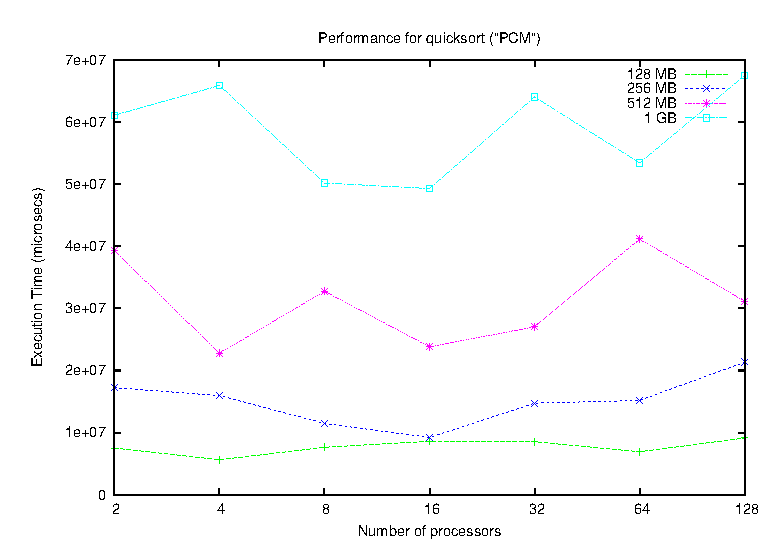
\includegraphics[width=0.4\textwidth]{plots/test_01_PCM/NxTxM/quicksort_PCM_NxTxM_large}} 
    \hspace*{20pt}  
    \subfloat[Bitonicsort.]{\label{NxTxM_large-bitonicsort}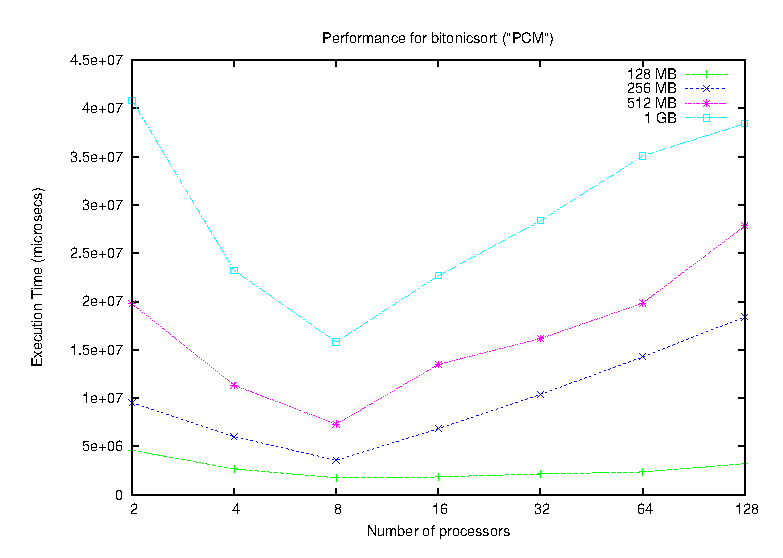
\includegraphics[width=0.4\textwidth]{plots/test_01_PCM/NxTxM/bitonicsort_PCM_NxTxM_large}} 
    
    \centering
    \subfloat[Bucketsort.]{\label{NxTxM_large-bucketsort}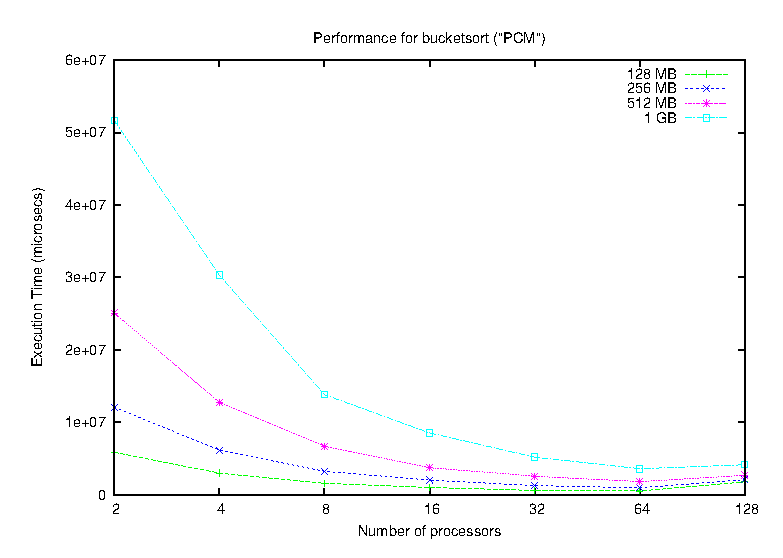
\includegraphics[width=0.4\textwidth]{plots/test_01_PCM/NxTxM/bucketsort_PCM_NxTxM_large}} 
    \hspace*{20pt}
    \subfloat[Samplesort.]{\label{NxTxM_large-samplesort}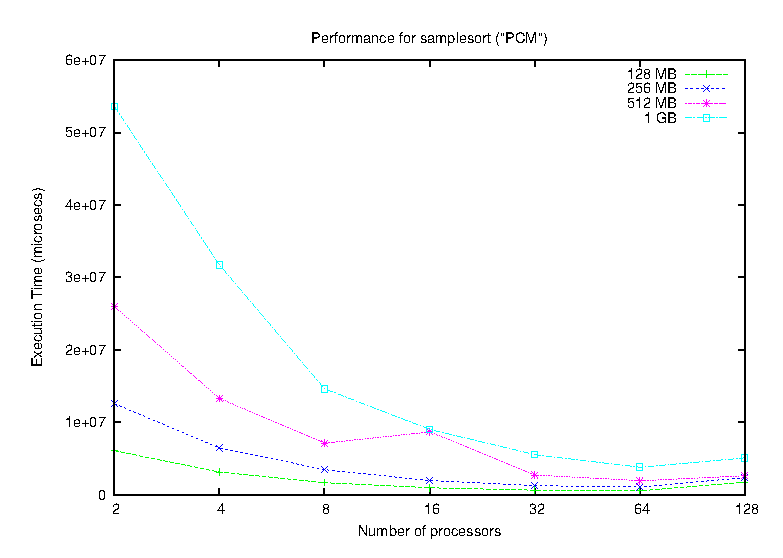
\includegraphics[width=0.4\textwidth]{plots/test_01_PCM/NxTxM/samplesort_PCM_NxTxM_large}} 
    
    \centering
    \subfloat[Mergesort.]{\label{NxTxM_large-mergesort}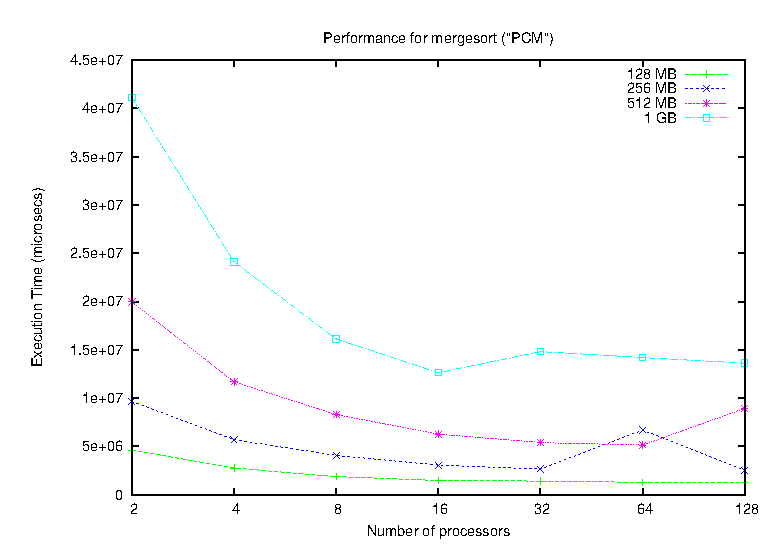
\includegraphics[width=0.4\textwidth]{plots/test_01_PCM/NxTxM/mergesort_PCM_NxTxM_large}}   
    \hspace*{20pt}  
    \subfloat[4-Way Mergesort.]{\label{NxTxM_large-kmerge}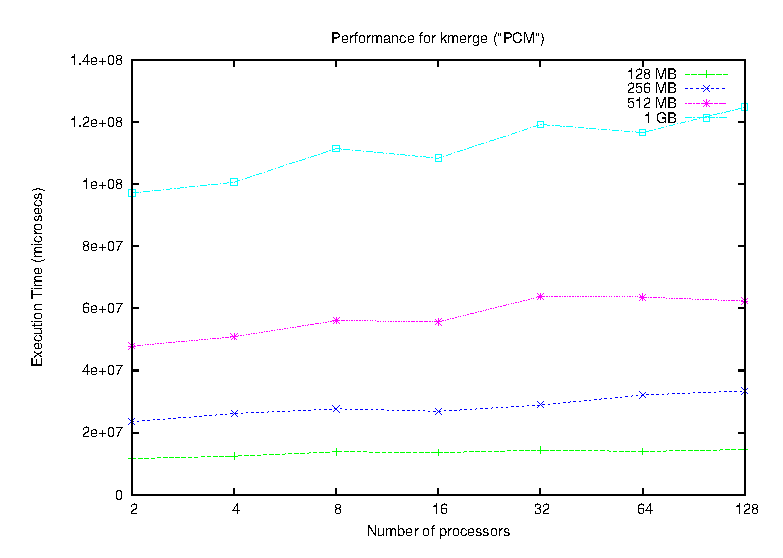
\includegraphics[width=0.4\textwidth]{plots/test_01_PCM/NxTxM/kmerge_PCM_NxTxM_large}} 
    
    \centering
    \subfloat[Load-Balanced Mergesort.]{\label{NxTxM_large-lbmergesort}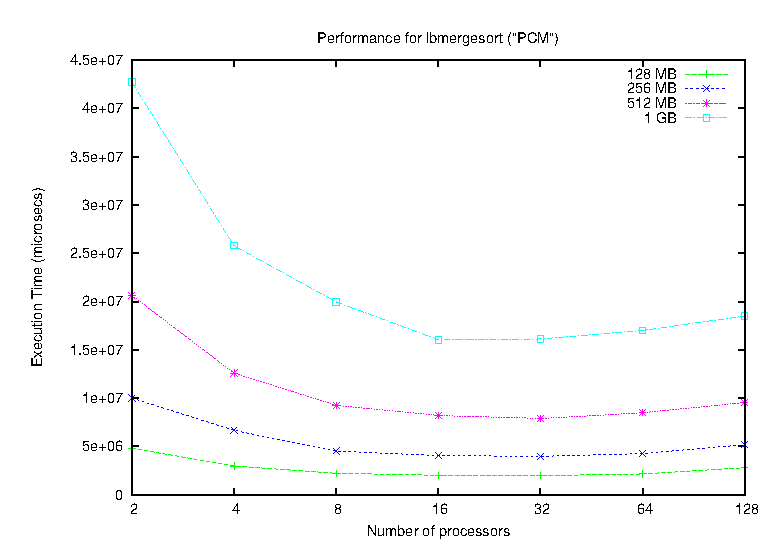
\includegraphics[width=0.4\textwidth]{plots/test_01_PCM/NxTxM/lbmergesort_PCM_NxTxM_large}} 
    \hspace*{20pt}  
    \subfloat[Load-Balanced Multi-Way Mergesort.]{\label{NxTxM_large-lbkmergesort}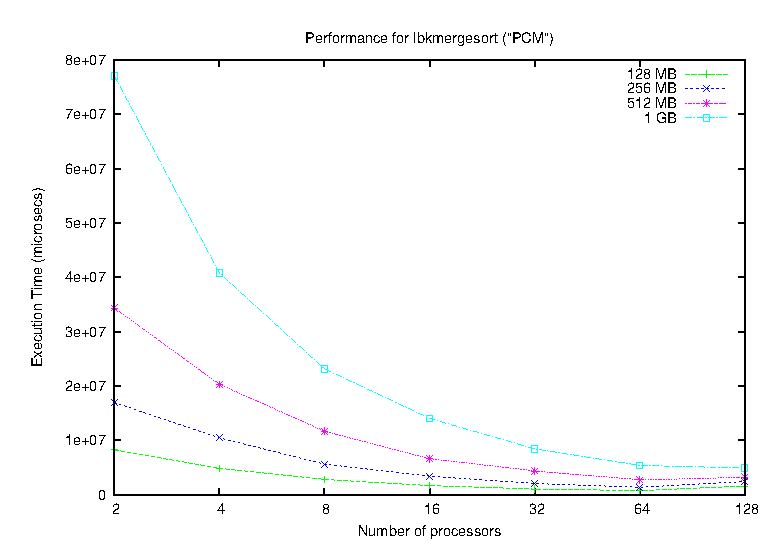
\includegraphics[width=0.4\textwidth]{plots/test_01_PCM/NxTxM/lbkmergesort_PCM_NxTxM_large}}  
    
\end{figure}
  



%%%%%%%%%%%%%%%%%%%%%%%%%%%%%%%%%%%%%%%% Huge data set %%%%%%%%%%%%%%%%%%%%%%%%%%%%%%%%%%%%%%%%%%%%%%%%%%%%%%
\begin{figure}[h]
	\ContinuedFloat
    \centering
    \subfloat[Quicksort.]{\label{NxTxM_huge-quicksort}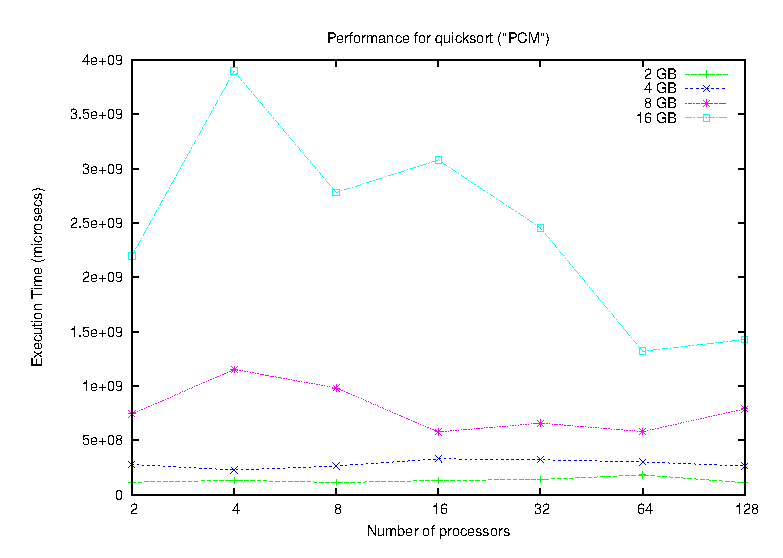
\includegraphics[width=0.4\textwidth]{plots/test_01_PCM/NxTxM/quicksort_PCM_NxTxM_huge}} 
    \hspace*{20pt}  
    \subfloat[Bitonicsort.]{\label{NxTxM_huge-bitonicsort}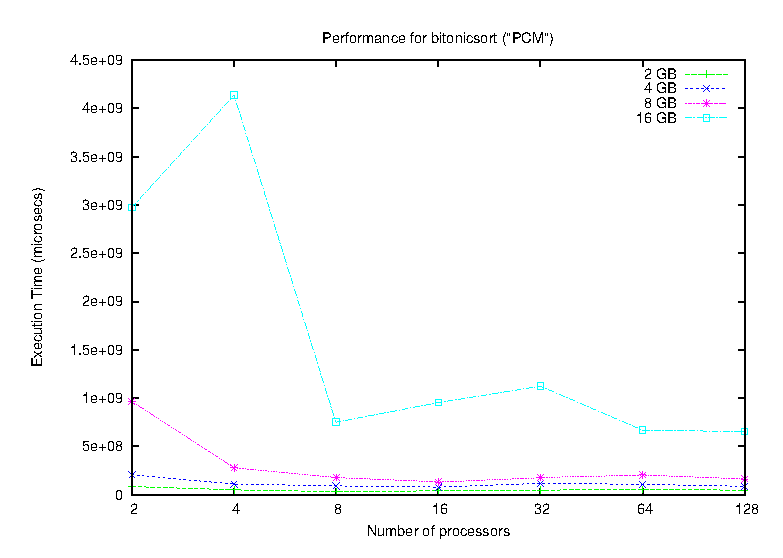
\includegraphics[width=0.4\textwidth]{plots/test_01_PCM/NxTxM/bitonicsort_PCM_NxTxM_huge}} 
    
    \centering
    \subfloat[Bucketsort.]{\label{NxTxM_huge-bucketsort}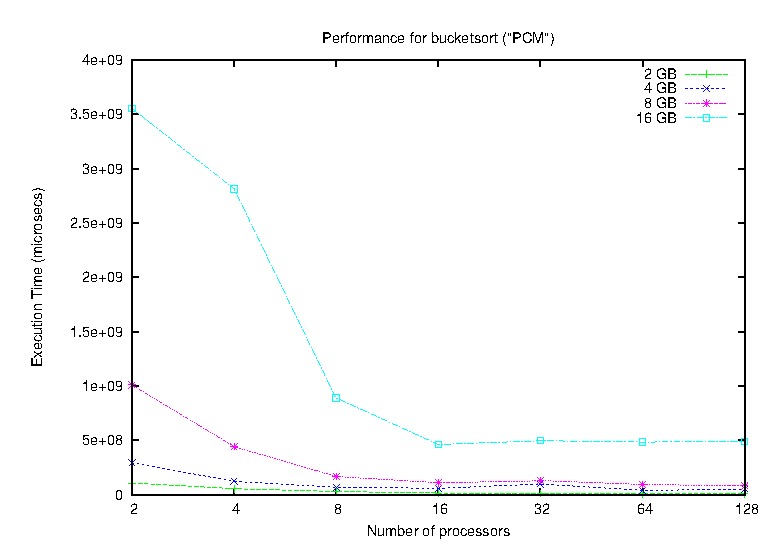
\includegraphics[width=0.4\textwidth]{plots/test_01_PCM/NxTxM/bucketsort_PCM_NxTxM_huge}} 
    \hspace*{20pt}
    \subfloat[Samplesort.]{\label{NxTxM_huge-samplesort}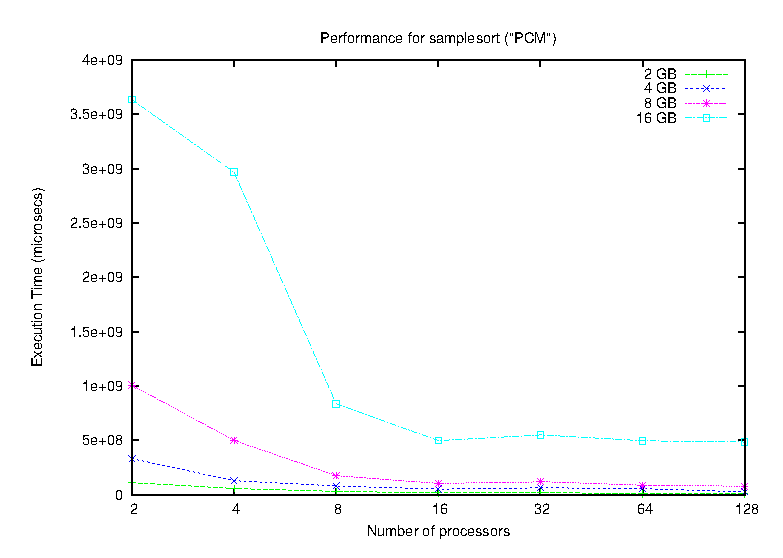
\includegraphics[width=0.4\textwidth]{plots/test_01_PCM/NxTxM/samplesort_PCM_NxTxM_huge}} 
    
    \centering
    \subfloat[Mergesort.]{\label{NxTxM_huge-mergesort}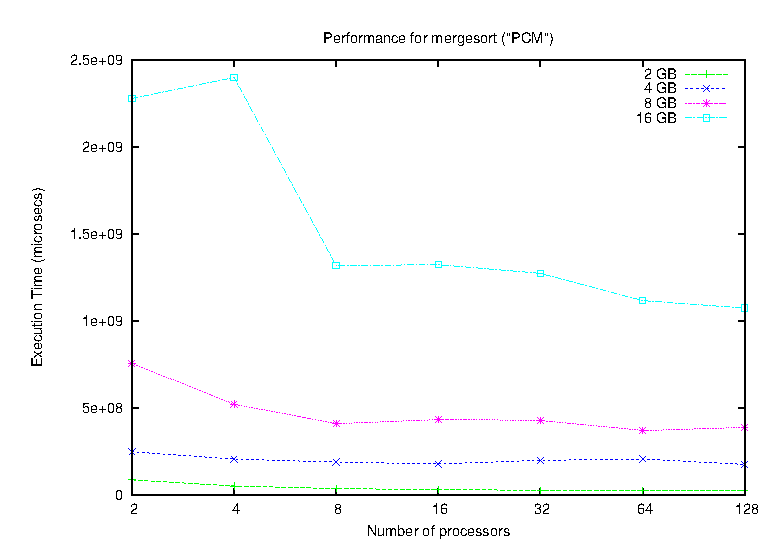
\includegraphics[width=0.4\textwidth]{plots/test_01_PCM/NxTxM/mergesort_PCM_NxTxM_huge}}   
    \hspace*{20pt}  
    \subfloat[4-Way Mergesort.]{\label{NxTxM_huge-kmerge}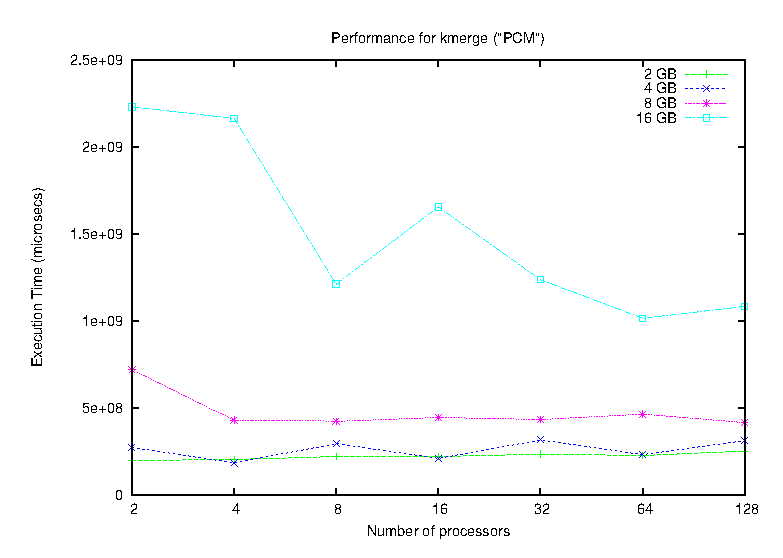
\includegraphics[width=0.4\textwidth]{plots/test_01_PCM/NxTxM/kmerge_PCM_NxTxM_huge}} 
    
    \centering
    \subfloat[Load-Balanced Mergesort.]{\label{NxTxM_huge-lbmergesort}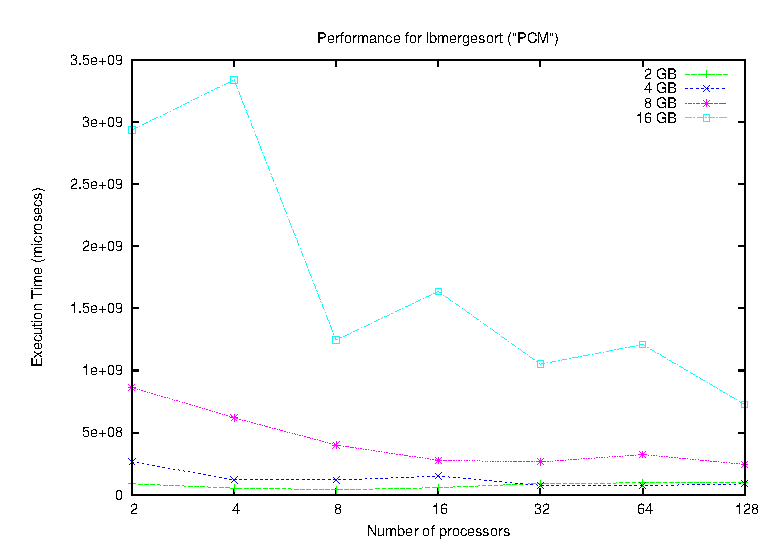
\includegraphics[width=0.4\textwidth]{plots/test_01_PCM/NxTxM/lbmergesort_PCM_NxTxM_huge}} 
    \hspace*{20pt}  
    \subfloat[Load-Balanced Multi-Way Mergesort.]{\label{NxTxM_huge-lbkmergesort}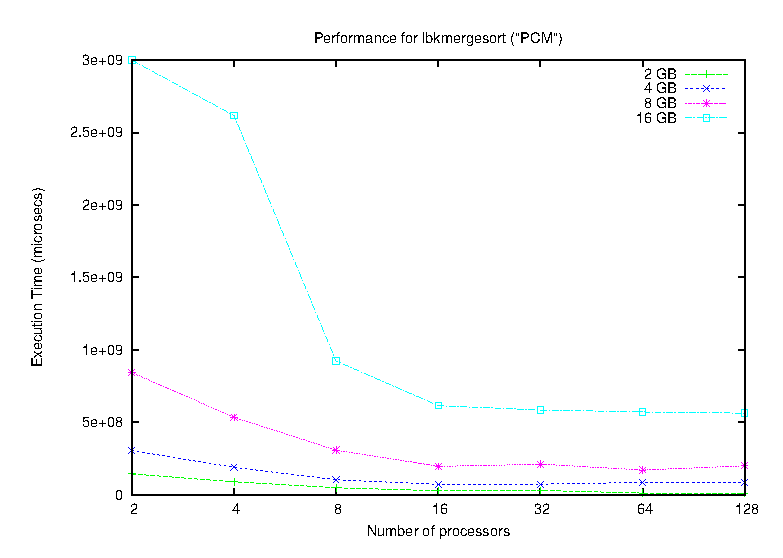
\includegraphics[width=0.4\textwidth]{plots/test_01_PCM/NxTxM/lbkmergesort_PCM_NxTxM_huge}}  
    
    \caption{\textit{PCM}. Time Completion of Sorting Algorithms by varying the parallelism degree. Each shape on a graphic represents the Time Completion of a certain Sorting Algorithm for a data set of specific size.}
    \label{NxTxM}
\end{figure}
  
  
\begin{figure}[!ht]
	\centering
	\subfloat[Quicksort.]{\label{MxTxN-quicksort}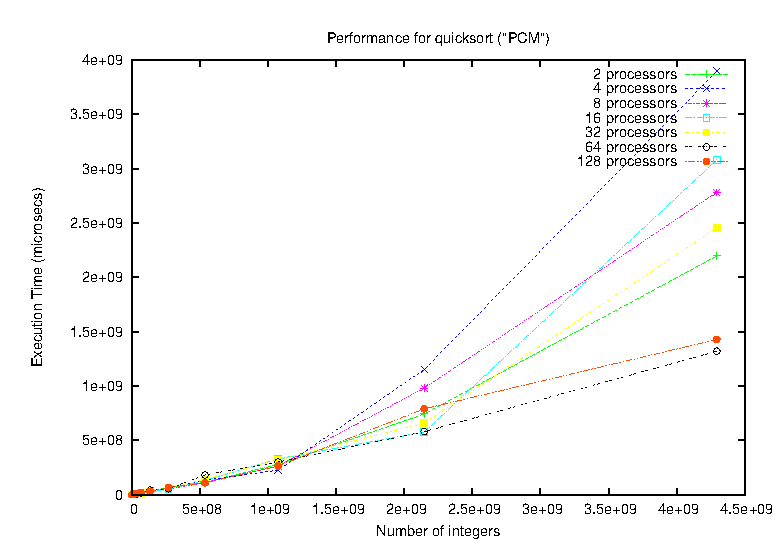
\includegraphics[width=0.4\textwidth]{plots/test_01_PCM/MxTxN/quicksort_PCM_MxTxN}} 
	\hspace*{20pt}	
  	\subfloat[Bitonicsort.]{\label{MxTxN-bitonicsort}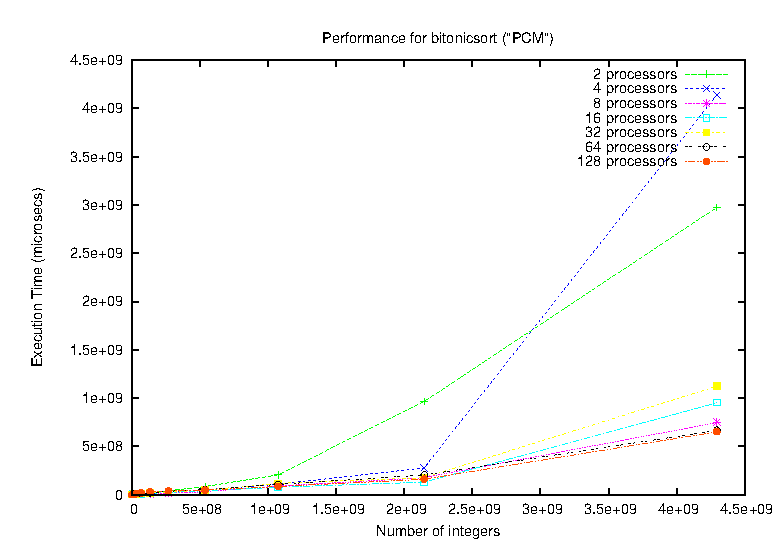
\includegraphics[width=0.4\textwidth]{plots/test_01_PCM/MxTxN/bitonicsort_PCM_MxTxN}} 
  		
	\centering
	\subfloat[Bucketsort.]{\label{MxTxN-bucketsort}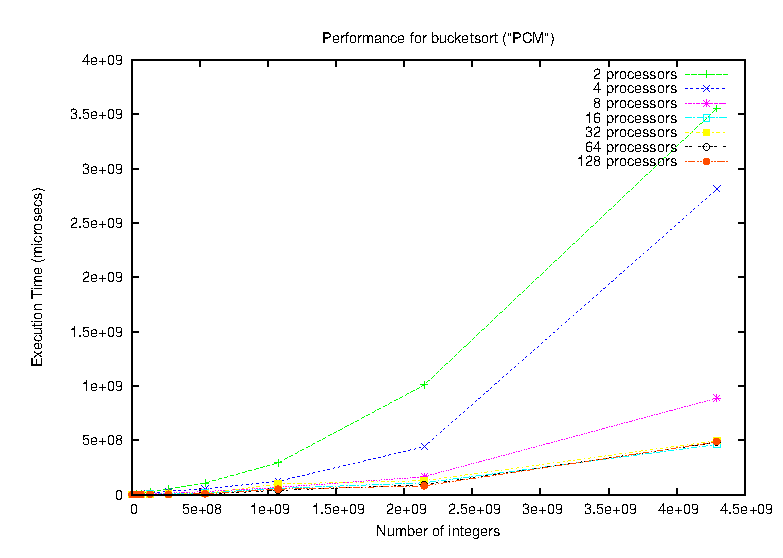
\includegraphics[width=0.4\textwidth]{plots/test_01_PCM/MxTxN/bucketsort_PCM_MxTxN}} 
  	\hspace*{20pt}
  	\subfloat[Samplesort.]{\label{MxTxN-samplesort}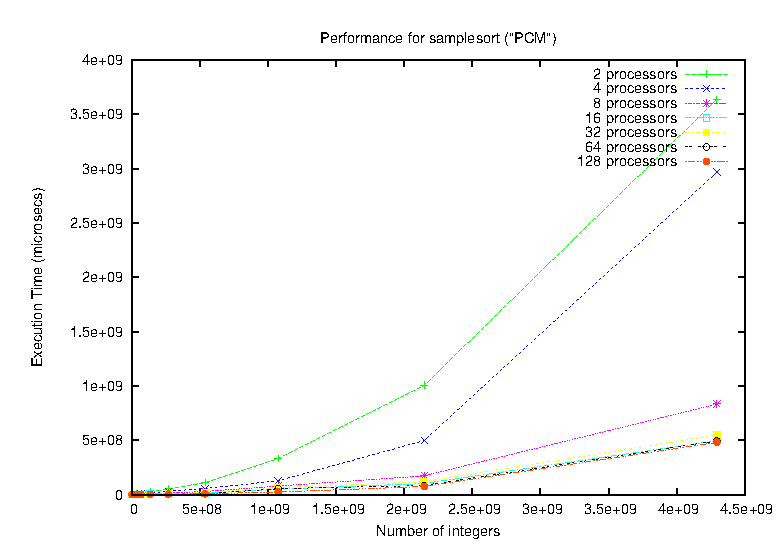
\includegraphics[width=0.4\textwidth]{plots/test_01_PCM/MxTxN/samplesort_PCM_MxTxN}} 
	
	\centering
  	\subfloat[Mergesort.]{\label{MxTxN-mergesort}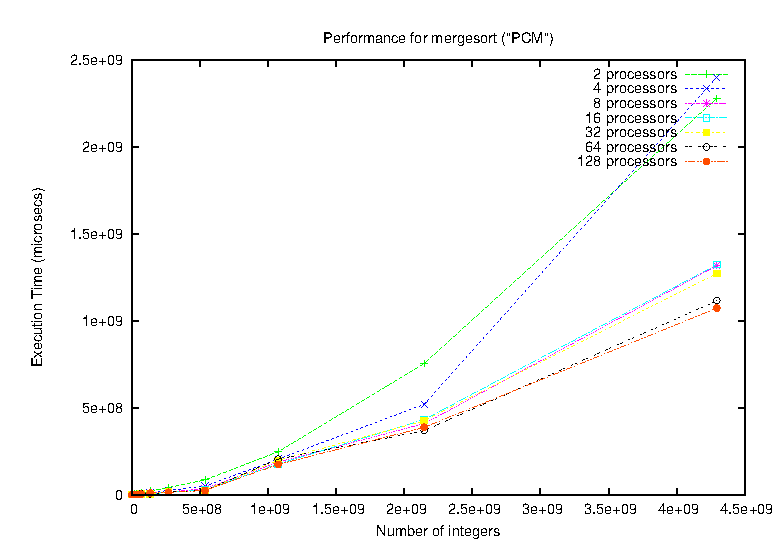
\includegraphics[width=0.4\textwidth]{plots/test_01_PCM/MxTxN/mergesort_PCM_MxTxN}}   
  	\hspace*{20pt}  
  	\subfloat[4-Way Mergesort.]{\label{MxTxN-kmerge}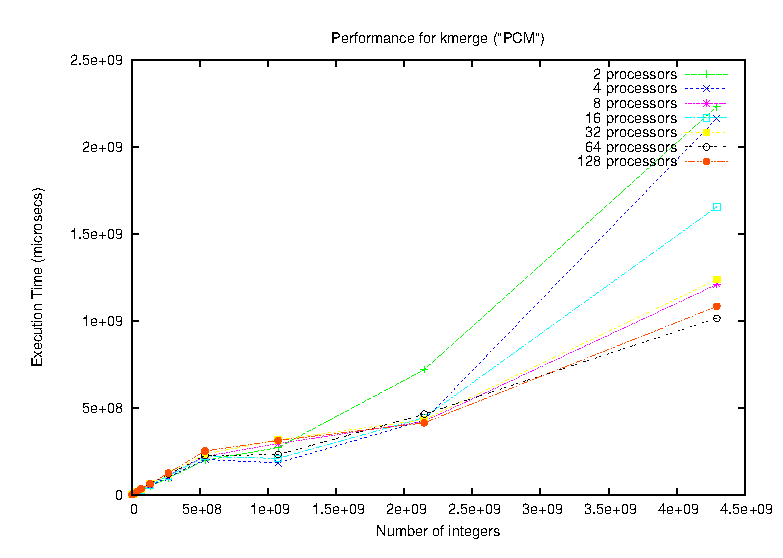
\includegraphics[width=0.4\textwidth]{plots/test_01_PCM/MxTxN/kmerge_PCM_MxTxN}} 
	
	\centering
  	\subfloat[Load-Balanced Mergesort.]{\label{MxTxN-lbmergesort}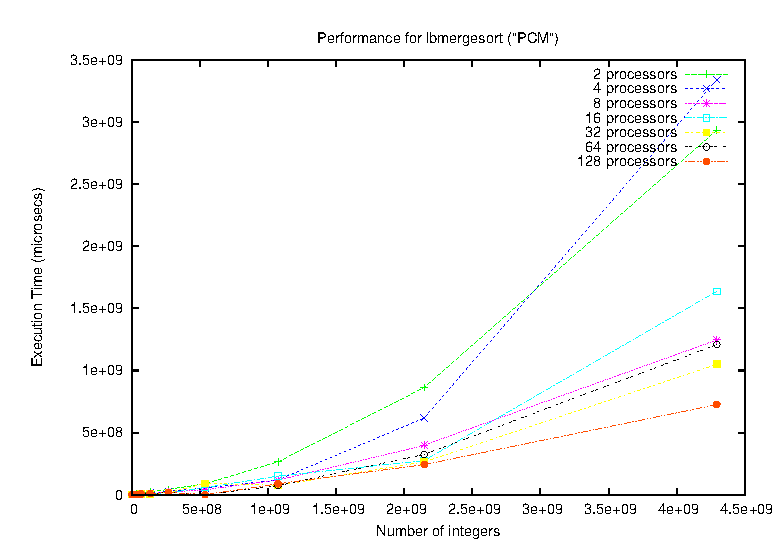
\includegraphics[width=0.4\textwidth]{plots/test_01_PCM/MxTxN/lbmergesort_PCM_MxTxN}} 
  	\hspace*{20pt}  
  	\subfloat[Load-Balanced Multi-Way Mergesort.]{\label{MxTxN-lbkmergesort}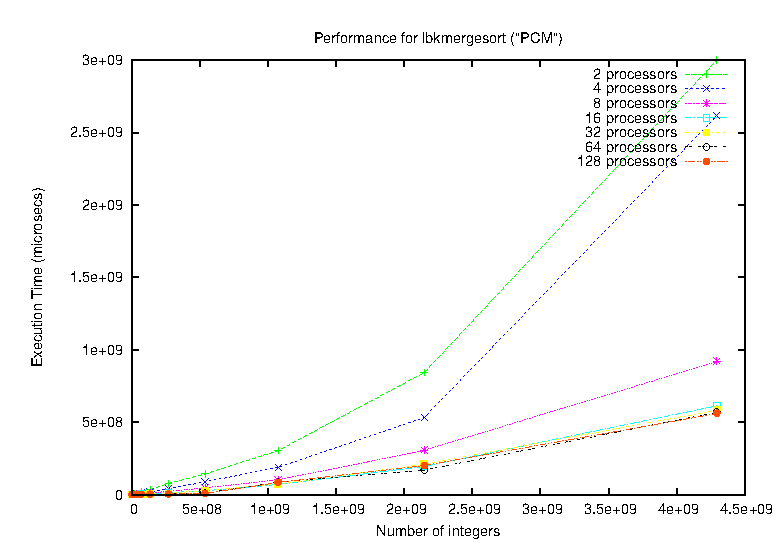
\includegraphics[width=0.4\textwidth]{plots/test_01_PCM/MxTxN/lbkmergesort_PCM_MxTxN}} 
  	
	\caption{\textit{PCM}. Time Completion of Sorting Algorithms for increasing sizes of the data set. }
	\label{MxTxN}
\end{figure} 
  
\paragraph{Comparison between Sorting Algorithms}
Figures~\ref{NxTxA-small},~\ref{NxTxA-large} and~\ref{NxTxA-huge} are useful to understand both which is the best algorithm to sort a specific data set, in terms of both absolute time completion and scalability. The distinction between small, large and huge data sets (corresponding to different computational grains) is still necessary to a better comparison. We first consider \textbf{small} and \textbf{large} data sets (Figure~\ref{NxTxA-small}). In general, the best time completion is obtained by \textit{Samplesort}, \textit{Bucketsort} and \textit{Load-balanced Multi-way Mergesort} at parallelism degree $n=64$; for $n=128$ the impact of communications together with smaller partitions bring to higher time completions (that is, time spent in sequential computation becomes relatively lower than the one spent in communications). Exactly as on $Pianosa$, \textit{Mergesort} confirm itself a ''good'' algorithm up to large data sets. \textit{Bitonicsort} is absolutely the ''strangest'' algorithm: it scales almost linear from $n=2$ to $n=4$ then, like most of other algorithms, keep improving up to $n=8$; finally, it starts worsen (for some data sets, the worsening is drastic) up to $n=128$. \textit{Bitonicsort} keeps this behavior even on large data sets, likely due to the increase of the communication cost outside $Infiniband$. Finally, we mention \textit{K-Way Mergesort} and \textit{Quicksort} that are the worst Sorting Algorithms on $PCM$: the former due to its "communication tree" which is pointlessly large in light of the small computational grain; the latter due to the unbalanced phases (see~\ref{appendixB} for more details). Moving to \textbf{huge} data sets, first annotation is necessarily for \textit{Bitonicsort}. We have explained its strange behavior on small and large data sets; now things are a little bit different, since the higher computational grain, enhanced by the fact that now the time spent in I/Os becomes meaningful, lead to a more smooth jump from $n=8$ to $n=16$. Best Sorting Algorithms are again \textit{Samplesort}, \textit{Bucketsort} and \textit{Load-balanced Multi-way Mergesort}; when the data set is of size $M=8GB$ or $M=16GB$, even the \textit{Bitonicsort} itself gets very close to these algorithms. However, we notice that, in general, when the data set is so huge, \textit{all} algorithms \textit{greatly} outperform the time completion of \textit{Sequentialsort} and tend to exhibit a better scalability. There are no evident reasons to think that this trend can change for higher data sets.

\begin{figure}[!ht]
	\centering
	\subfloat[Data set of 1M integers.]{\label{NxTxA-1M}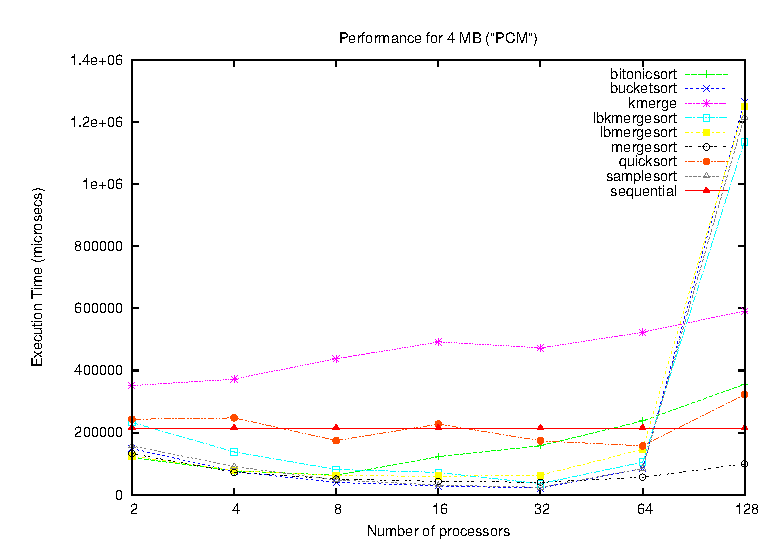
\includegraphics[width=0.4\textwidth]{plots/test_01_PCM/NxTxA/M1048576_PCM_NxTxA}} 
	\hspace*{20pt}	
  	\subfloat[Data set of 2M integers.]{\label{NxTxA-2M}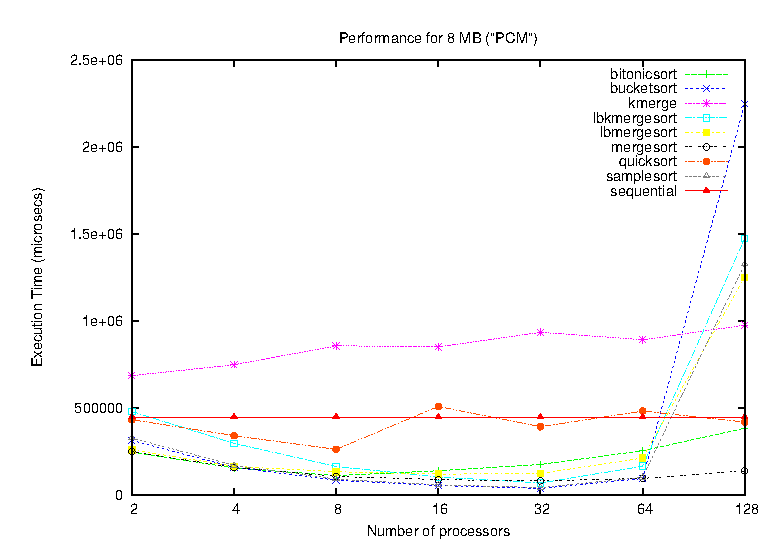
\includegraphics[width=0.4\textwidth]{plots/test_01_PCM/NxTxA/M2097152_PCM_NxTxA}} 
  		
	\centering
	\subfloat[Data set of 4M integers.]{\label{NxTxA-4M}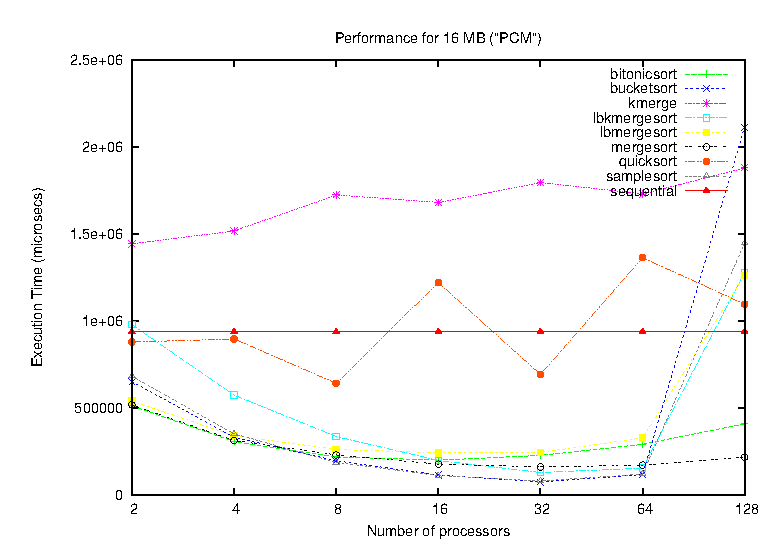
\includegraphics[width=0.4\textwidth]{plots/test_01_PCM/NxTxA/M4194304_PCM_NxTxA}} 
  	\hspace*{20pt}
  	\subfloat[Data set of 8M integers.]{\label{NxTxA-8M}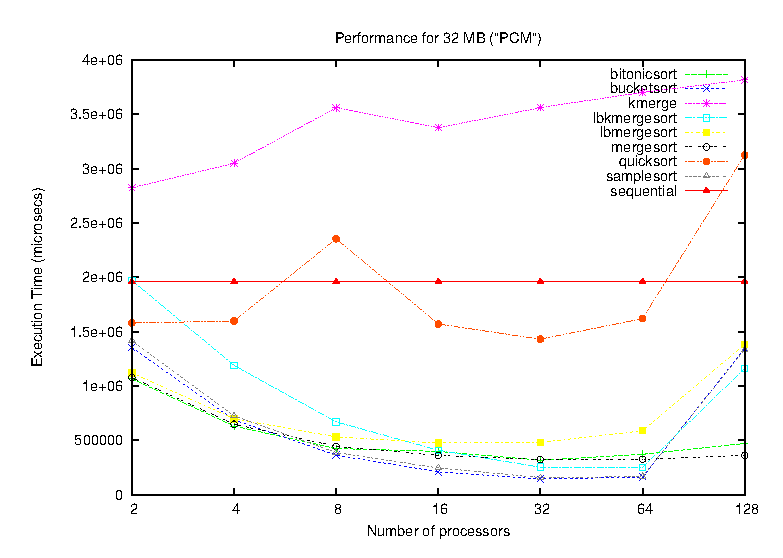
\includegraphics[width=0.4\textwidth]{plots/test_01_PCM/NxTxA/M8388608_PCM_NxTxA}} 
	
	\centering
  	\subfloat[Data set of 16M integers.]{\label{NxTxA-16M}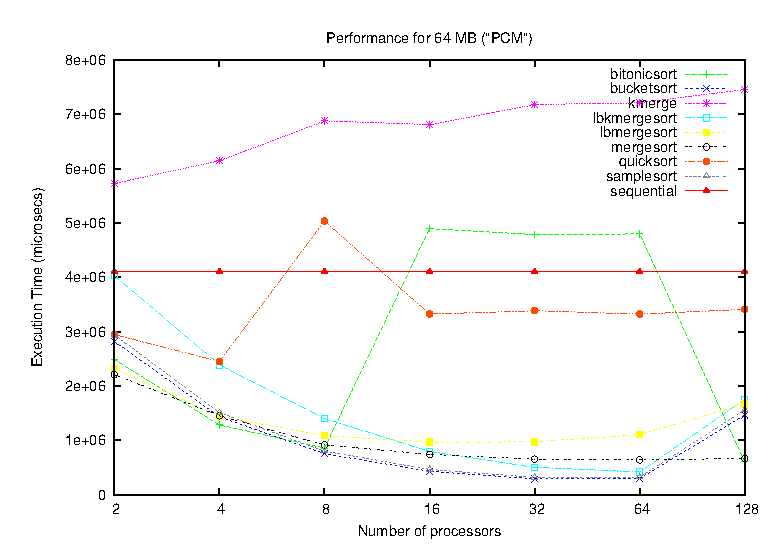
\includegraphics[width=0.4\textwidth]{plots/test_01_PCM/NxTxA/M16777216_PCM_NxTxA}}   
  	\hspace*{20pt}  
  	\subfloat[Data set of 32M integers.]{\label{NxTxA-32M}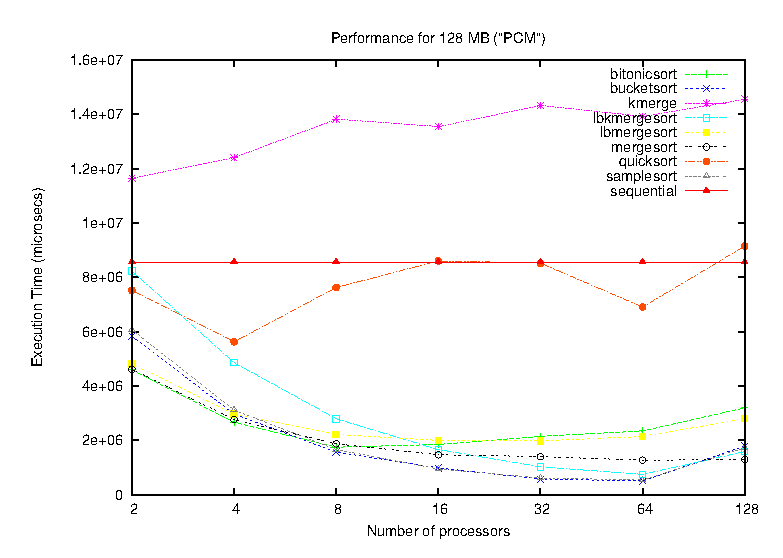
\includegraphics[width=0.4\textwidth]{plots/test_01_PCM/NxTxA/M33554432_PCM_NxTxA}} 
  	
	\caption{\textit{PCM}. Time Completion for sorting \textit{small} data sets. Each graphic represents a data set of fixed size, while each shape on a graphic shows the Time Completion of a certain Sorting Algorithm for that data set.}
	\label{NxTxA-small}
\end{figure} 

\begin{figure}[!ht]
	\centering
	\subfloat[Data set of 64M integers.]{\label{NxTxA-64M}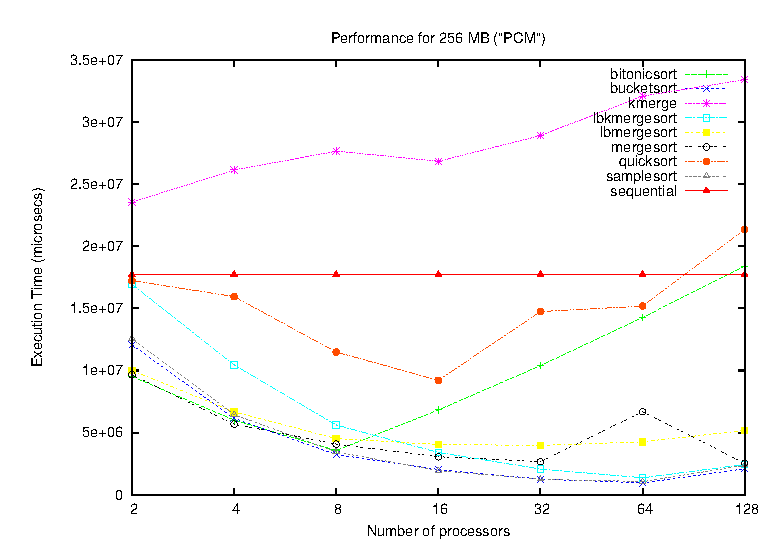
\includegraphics[width=0.5\textwidth]{plots/test_01_PCM/NxTxA/M67108864_PCM_NxTxA}} 
	
	\centering
  	\subfloat[Data set of 128M integers.]{\label{NxTxA-128M}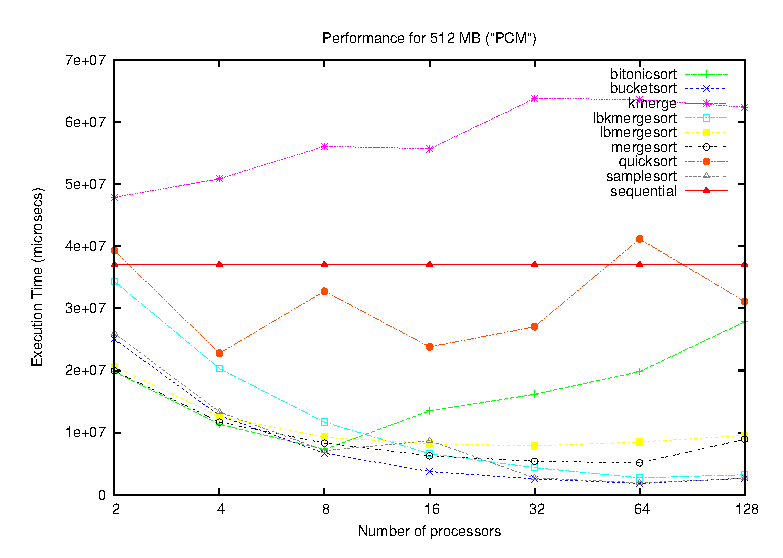
\includegraphics[width=0.5\textwidth]{plots/test_01_PCM/NxTxA/M134217728_PCM_NxTxA}} 
  		
	\centering
	\subfloat[Data set of 256M integers.]{\label{NxTxA-256M}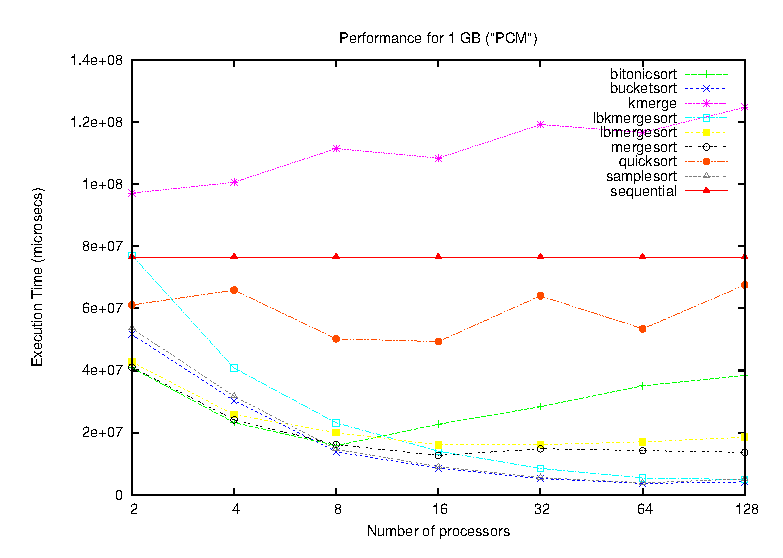
\includegraphics[width=0.5\textwidth]{plots/test_01_PCM/NxTxA/M268435456_PCM_NxTxA}} 
  	
  	\caption{\textit{PCM}. Time Completion for sorting \textit{large} data sets. Each graphic represents a data set of fixed size, while each shape on a graphic shows the Time Completion of a certain Sorting Algorithm for that data set.}
	\label{NxTxA-large}
\end{figure}

\begin{figure}[!ht]  	
  	\centering
  	\subfloat[Data set of 512M integers.]{\label{NxTxA-512M}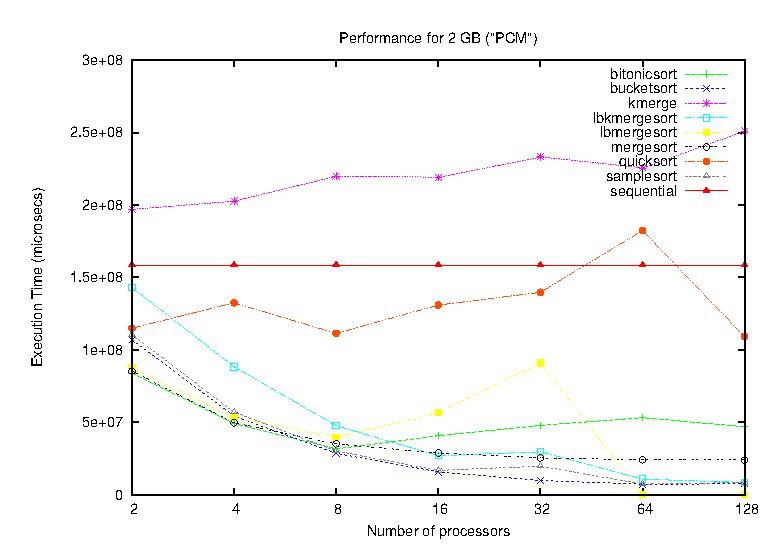
\includegraphics[width=0.4\textwidth]{plots/test_01_PCM/NxTxA/M536870912_PCM_NxTxA}} 
	\hspace*{20pt}  
  	\subfloat[Data set of 1G integers.]{\label{NxTxA-1G}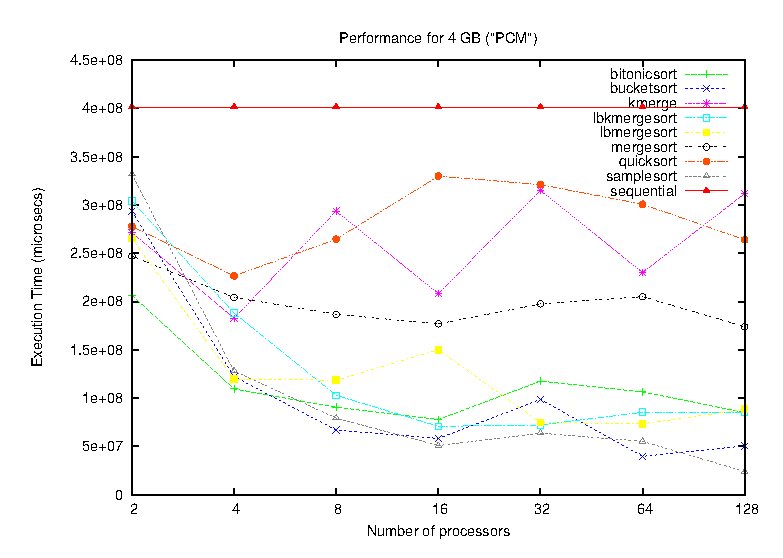
\includegraphics[width=0.4\textwidth]{plots/test_01_PCM/NxTxA/M1073741824_PCM_NxTxA}}   
	
	\centering
  	\subfloat[Data set of 2G integers.]{\label{NxTxA-2G}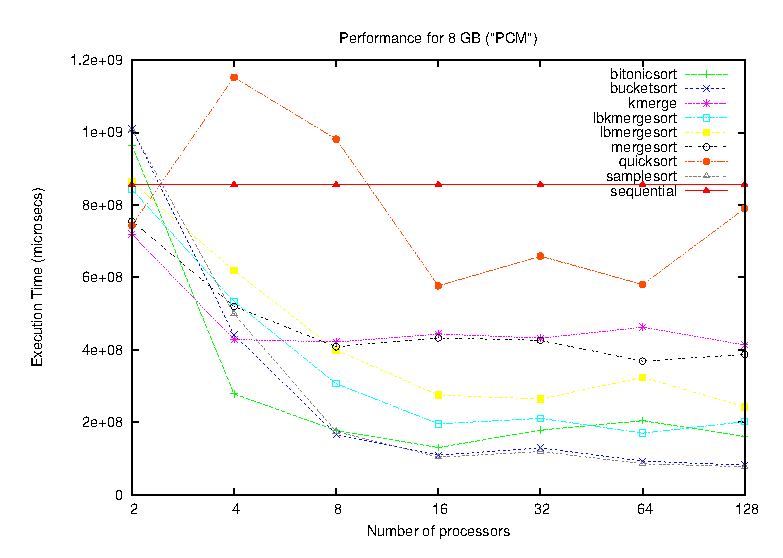
\includegraphics[width=0.4\textwidth]{plots/test_01_PCM/NxTxA/M2147483648_PCM_NxTxA}}  
	\hspace*{20pt}  
  	\subfloat[Data set of 4G integers.]{\label{NxTxA-4G}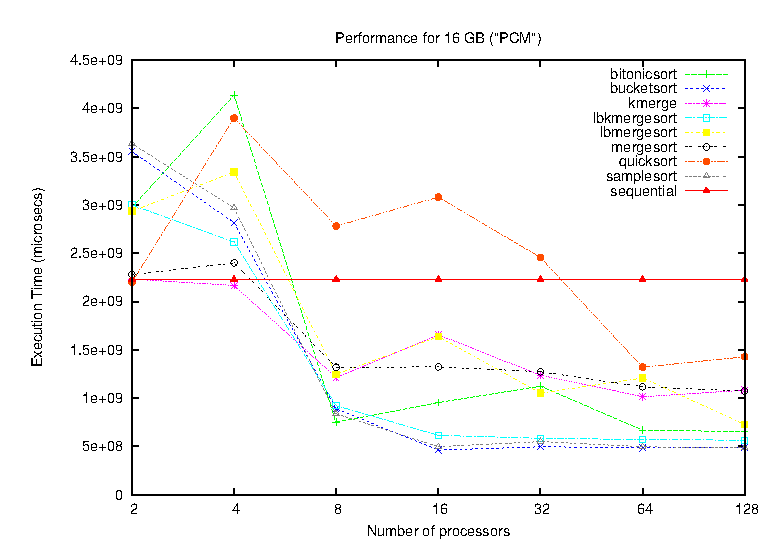
\includegraphics[width=0.4\textwidth]{plots/test_01_PCM/NxTxA/M4294967296_PCM_NxTxA}}   
  	
	\caption{\textit{PCM}. Time Completion for sorting \textit{huge} data sets. Each graphic represents a data set of fixed size, while each shape on a graphic shows the Time Completion of a certain Sorting Algorithm for that data set.}
	\label{NxTxA-huge}
\end{figure} 

\begin{figure}[!ht]
	\centering
	\subfloat[Parallelism degree 2.]{\label{MxTxA-n2}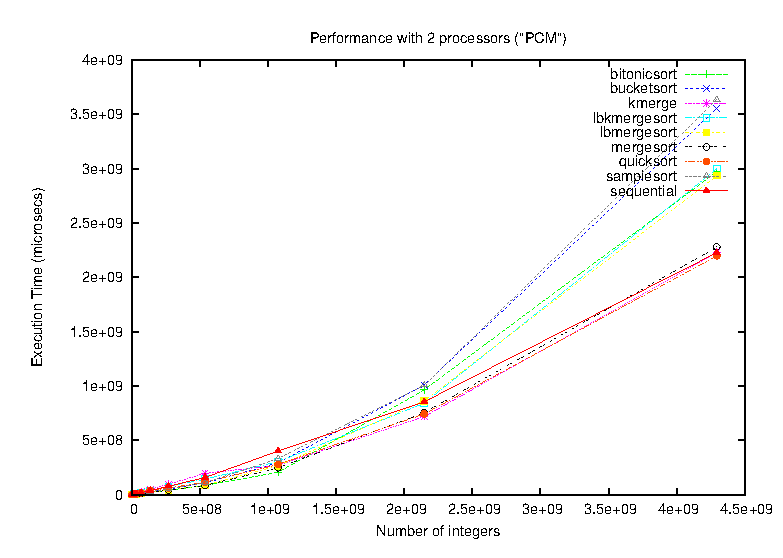
\includegraphics[width=0.4\textwidth]{plots/test_01_PCM/MxTxA/n2_PCM_MxTxA}} 
	\hspace*{20pt}	
  	\subfloat[Parallelism degree 4.]{\label{MxTxA-n4}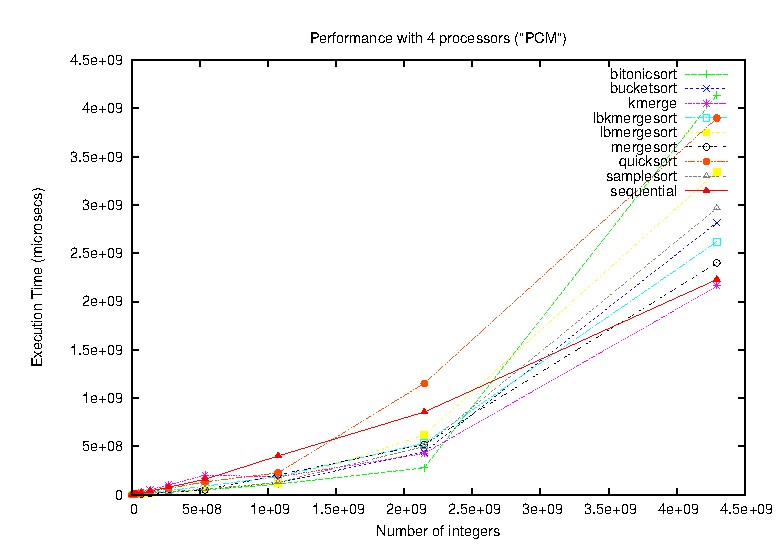
\includegraphics[width=0.4\textwidth]{plots/test_01_PCM/MxTxA/n4_PCM_MxTxA}} 
  		
	\centering
	\subfloat[Parallelism degree 8.]{\label{MxTxA-n8}\includegraphics[width=0.4\textwidth]{plots/test_01_PCM/MxTxA/n8_PCM_MxTxA}} 
  	\hspace*{20pt}
  	\subfloat[Parallelism degree 16.]{\label{MxTxA-n16}\includegraphics[width=0.4\textwidth]{plots/test_01_PCM/MxTxA/n16_PCM_MxTxA}} 
  		
	\centering
	\subfloat[Parallelism degree 32.]{\label{MxTxA-n32}\includegraphics[width=0.4\textwidth]{plots/test_01_PCM/MxTxA/n32_PCM_MxTxA}} 
  	\hspace*{20pt}
  	\subfloat[Parallelism degree 64.]{\label{MxTxA-n64}\includegraphics[width=0.4\textwidth]{plots/test_01_PCM/MxTxA/n64_PCM_MxTxA}} 
  	
	\centering
	\subfloat[Parallelism degree 128.]{\label{MxTxA-n128}\includegraphics[width=0.4\textwidth]{plots/test_01_PCM/MxTxA/n128_PCM_MxTxA}} 
  	
	\caption{\textit{PCM}. Time Completion for sorting data sets with fixed parallelism degree.}
	\label{MxTxA}
\end{figure} 

\clearpage